% report.tex
%
% Purpose:
%   Main LaTeX driver for a first-draft technical report on the boundary
%   integral trace-subspace formulation used in this repository.
%
% Main workflow:
%   The report is split into six paper-style section files under sections/.
%   It introduces the model and notation, develops the trace-subspace
%   formulation, records the numerical discretization and implementation
%   workflow, and leaves a standard placeholder for numerical experiments.
%
% Based on:
%   notes/theory/scat_formulation.md, notes/theory/scat_formulation2.md,
%   notes/theory/mode_selection.md, notes/theory/bloch_mode.md,
%   notes/implementation/kress_quadrature.md, notes/implementation/kress_scheme.md,
%   notes/implementation/mfs2d.md, and pre/pre1/pre1.tex.
%
% Main changes:
%   The report uses a compact paper-like organization rather than one top-level
%   section per concept.  The detailed derivations are grouped into subsections.
%
% Numerical goal:
%   Provide a readable, compilable reference document for the current
%   Transmission Eigenvalue / Bloch-mode / line-defect implementation workflow.

\documentclass[11pt]{article}

\usepackage[margin=1in]{geometry}
\usepackage{amsmath}
\usepackage{amssymb}
\usepackage{amsthm}
\usepackage{mathtools}
\usepackage{bm}
\usepackage{graphicx}
\usepackage{tikz}
\usepackage{url}
\usepackage[hidelinks]{hyperref}

\usetikzlibrary{arrows.meta}

\newcommand{\ii}{\mathrm{i}}
\newcommand{\ee}{\mathrm{e}}
\newcommand{\dd}{\mathrm{d}}
\newcommand{\CC}{\mathbb C}
\newcommand{\RR}{\mathbb R}
\newcommand{\Ccell}{\mathcal C}
\newcommand{\Tspace}{\mathcal T}
\newcommand{\Aqp}{A_{\mathrm{QP}}}
\newcommand{\Asc}{A_{\mathrm{sc}}}
\newcommand{\Bsc}{B_{\mathrm{sc}}}
\newcommand{\Atr}{\mathcal A}
\newcommand{\Ein}{E_{\mathrm{in}}}
\newcommand{\Eout}{E_{\mathrm{out}}}
\newcommand{\Din}{D_{\mathrm{in}}}
\newcommand{\Nin}{N_{\mathrm{in}}}
\newcommand{\Dout}{D_{\mathrm{out}}}
\newcommand{\Nout}{N_{\mathrm{out}}}
\newcommand{\sigmin}{\sigma_{\min}}
\newcommand{\GammaR}{\Gamma_{\mathrm R}}
\newcommand{\FigurePlaceholder}[1]{%
  \begin{center}
    \setlength{\fboxsep}{1.2em}%
    \fbox{\parbox{0.75\textwidth}{\centering #1}}%
  \end{center}%
}
\newcommand{\SafeIncludeGraphics}[2][]{%
  \IfFileExists{#2}{%
    \includegraphics[#1]{#2}%
  }{%
    \FigurePlaceholder{Missing figure: \url{#2}}%
  }%
}
\DeclareMathOperator{\diag}{diag}
\DeclareMathOperator{\rank}{rank}

\title{A Boundary Integral Trace-Subspace Formulation for Periodic Line-Defect Waveguides}
\author{Draft technical note}
\date{\today}

\begin{document}

\maketitle

\begin{abstract}
This note records a constructive numerical formulation for periodic line-defect
scattering and eigenvalue calculations in a two-dimensional scalar Helmholtz
transmission model.  The formulation combines boundary integral equations on
material interfaces, compact quasiperiodic port traces, Rayleigh coordinate
spaces, one-cell Bloch/scattering computations in the periodic half-leads, and a
center-cell trace-matching system.  The main point is not to construct the full
periodic half-guide Dirichlet-to-Neumann map explicitly, but to impose the
finite-dimensional Cauchy trace subspace selected by the Bloch-mode radiation or
admissibility condition.  The document is a first draft intended to make the
current implementation readable and testable.
\end{abstract}

\tableofcontents

% 01_introduction.tex
%
% Purpose:
%   Introduce the line-defect waveguide problem, the constructive trace-subspace
%   method, and the relation to existing quasiperiodic BIE and periodic
%   waveguide boundary-condition literature.
%
% Main algorithm:
%   This section is expository.  It states the computational objective and
%   positions the formulation before the mathematical details are introduced.
%
% Based on:
%   sections/intro.tex from the first report draft and pre/pre1/pre1.tex.
%
% Main changes:
%   Keeps the motivation and literature discussion at the top level while
%   moving detailed geometry and trace notation to the preliminaries.
%
% Numerical goal:
%   Clarify what the report is meant to support: scattering solves, homogeneous
%   singular-value scans, and future numerical validation.

\section{Introduction}

This report develops a constructive numerical realization for periodic
line-defect waveguide scattering and eigenvalue-type calculations.  The model is
a scalar Helmholtz transmission problem in a two-dimensional geometry that is
quasiperiodic in the transverse direction and open through periodic half-leads
in the longitudinal direction.  The two main workflows are forced lead
scattering, where incoming Bloch data are prescribed from one or both leads, and
homogeneous eigenvalue or transmission-eigenvalue-type searches, where a
nontrivial admissible null vector is sought.

The formulation combines several standard numerical ingredients in a compact
port framework: boundary integral equations on material interfaces, artificial
quasiperiodic ports, Rayleigh coordinates for wall Cauchy traces, one-cell
scattering computations in the periodic leads, Bloch-mode selection of
incoming/outgoing trace subspaces, and a center-cell matching system.  Its main
point is not to construct a new abstract Dirichlet-to-Neumann theory for
periodic half-guides.  Instead, it builds the finite-dimensional Cauchy trace
subspaces needed by the current line-defect geometry and imposes those
subspaces directly in the global matrix.

The distinction between coordinates and physics is central.  Rayleigh modes form
a convenient Fourier basis for traces on a vertical port, but an arbitrary
Rayleigh Cauchy vector need not be the trace of an admissible half-lead solution.
Physical incoming and outgoing data are identified by a lead-cell Bloch or
scattering computation, followed by a mode-selection rule.  Once the admissible
subspace has been selected, any numerically well-conditioned basis of that same
subspace may be used in the coupled system.

\subsection{Relation to existing methods}

The present formulation is closely related to several established strands of
work.  Boundary integral methods for quasiperiodic band-structure calculations,
including the numerical difficulties associated with quasiperiodic Green
functions and empty-cell resonances, are represented by the work of Barnett and
Greengard \cite{BarnettGreengard2010}.  Exact boundary conditions for locally
perturbed periodic waveguides are developed by Joly, Li, and Fliss
\cite{JolyLiFliss2006}, where half-guide exterior conditions are described
through periodic-guide Dirichlet-to-Neumann and related operators.  Coatl\'even
\cite{Coatleven2012} treats Helmholtz problems in periodic media with line
defects using a combination of Floquet--Bloch transforms,
Lippmann--Schwinger ideas, and Dirichlet-to-Neumann maps.

The present formulation differs from these approaches in emphasis.  It is a
compact-port finite-dimensional trace-space realization tailored to the current
boundary integral implementation.  It should not be read as replacing the full
functional-analytic half-guide theory.  Rather, it records how Rayleigh wall
coordinates, one-cell Bloch/scattering calculations, and center-cell boundary
integral equations are assembled into a practical matrix formulation whose
truncation and mode-selection choices can be tested numerically.

% 02_preliminaries.tex
%
% Purpose:
%   Collect geometry, quasiperiodicity, the scalar transmission model, Rayleigh
%   trace coordinates, and the two global workflows before the main
%   trace-subspace formulation.
%
% Main algorithm:
%   This section defines the variables, function spaces, and matrix problem
%   types used later.  It does not introduce the lead-cell Bloch algorithm.
%
% Based on:
%   sections/intro.tex, sections/problem.tex, and sections/trace_spaces.tex from
%   the first report draft.
%
% Main changes:
%   Moves geometry and Rayleigh coordinates out of separate top-level sections
%   and places them under a standard preliminaries section.
%
% Numerical goal:
%   Fix the notation used by the matrix assembly and validation workflow.

\section{Preliminaries}

\subsection{Geometry and quasiperiodicity}

The longitudinal lead direction is \(x\).  The transverse quasiperiodic
direction is \(y\), with period \(d\).  The field satisfies
\[
  u(x,y+d)=\ee^{\ii\beta d}u(x,y),
\]
where \(\beta\) is the transverse quasimomentum.  The three reference cells
nearest the defect are
\[
  \Ccell^-,
  \qquad
  \Ccell^0,
  \qquad
  \Ccell^+ .
\]
The center obstacle is \(\Omega_0\), with boundary
\[
  \Sigma=\partial\Omega_0 .
\]
The adjacent lead obstacles are denoted \(\Omega_-\) and \(\Omega_+\).  The
artificial center-cell ports are
\[
  \Gamma_-=\{x=X_-\},
  \qquad
  \Gamma_+=\{x=X_+\}.
\]
Their outward normals, always taken with respect to the center cell, are
\[
  \nu_{\Gamma_-}=-e_x,
  \qquad
  \nu_{\Gamma_+}=+e_x .
\]
When the longitudinal periods of the two half-leads are needed, they are written
\(L_-\) and \(L_+\).  The symbol \(d\) is reserved for the transverse
quasiperiodic period.

\begin{figure}[ht]
\centering
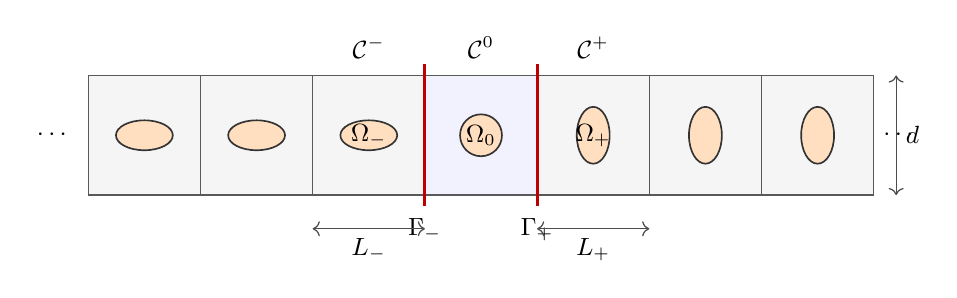
\begin{tikzpicture}[
  x=0.95cm,
  y=0.95cm,
  every node/.style={font=\small},
  cell/.style={draw=black!65, line width=0.5pt},
  leadcell/.style={fill=gray!8},
  centercell/.style={fill=blue!5},
  inclusion/.style={draw=black!80, fill=orange!25, line width=0.6pt},
  port/.style={draw=red!75!black, line width=1.1pt},
  dim/.style={<->, draw=black!70, line width=0.45pt}
]
  \foreach \x in {-5.25,-3.75,-2.25} {
    \draw[cell, leadcell] (\x,-0.8) rectangle ++(1.5,1.6);
    \draw[inclusion] (\x+0.75,0) ellipse [x radius=0.38, y radius=0.20];
  }

  \draw[cell, centercell] (-0.75,-0.8) rectangle (0.75,0.8);
  \draw[inclusion] (0,0) circle [radius=0.28];

  \foreach \x in {0.75,2.25,3.75} {
    \draw[cell, leadcell] (\x,-0.8) rectangle ++(1.5,1.6);
    \draw[inclusion] (\x+0.75,0) ellipse [x radius=0.22, y radius=0.38];
  }

  \draw[port] (-0.75,-0.95) -- (-0.75,0.95);
  \draw[port] (0.75,-0.95) -- (0.75,0.95);

  \node[above] at (-1.5,0.9) {$\mathcal C^-$};
  \node[above] at (0,0.9) {$\mathcal C^0$};
  \node[above] at (1.5,0.9) {$\mathcal C^+$};

  \node[below] at (-0.75,-0.98) {$\Gamma_-$};
  \node[below] at (0.75,-0.98) {$\Gamma_+$};

  \node at (-1.5,0) {$\Omega_-$};
  \node at (0,0) {$\Omega_0$};
  \node at (1.5,0) {$\Omega_+$};

  \draw[dim] (-2.25,-1.25) -- (-0.75,-1.25);
  \node[below] at (-1.5,-1.25) {$L_-$};
  \draw[dim] (0.75,-1.25) -- (2.25,-1.25);
  \node[below] at (1.5,-1.25) {$L_+$};

  \draw[dim] (5.55,-0.8) -- (5.55,0.8);
  \node[right] at (5.55,0) {$d$};
  \node[left] at (-5.35,0) {$\cdots$};
  \node[right] at (5.25,0) {$\cdots$};
\end{tikzpicture}
\caption{Schematic of the center cell, adjacent periodic lead cells, and compact
ports.  The diagram is not a geometry specification; the actual inclusion shapes
are supplied by the geometry routines.}
\label{fig:cells}
\end{figure}

\subsection{Helmholtz transmission problem}

In each homogeneous material region the field satisfies a scalar Helmholtz
equation.  In the exterior background and inside an inclusion we write
\[
  (\Delta+k_e^2)u_e=0,
  \qquad
  (\Delta+k_i^2)u_i=0 .
\]
For a dielectric inclusion with relative index \(n\), one often has
\(k_i=nk_e\), but the formulation only uses the exterior and interior
wavenumbers supplied to the boundary integral assembly.

Across a smooth material interface \(\Sigma_j=\partial\Omega_j\), the TM-like
transmission conditions used in the current formulation are
\[
  u_e=u_i,
  \qquad
  \partial_\nu u_e=\partial_\nu u_i .
\]
Here \(\nu\) is the unit normal pointing out of the inclusion.  A TE variant
would replace the Neumann continuity by a weighted normal derivative condition,
but that is a change in the boundary condition row rather than in the
trace-subspace idea.

\subsection{Rayleigh trace coordinates}

On a vertical port \(x=X\), the transverse quasiperiodicity suggests the
Rayleigh basis
\[
  \beta_m=\beta+\frac{2\pi m}{d},
  \qquad
  \psi_m(y)=\frac{1}{\sqrt d}\ee^{\ii\beta_m y},
  \qquad
  m\in\mathbb Z .
\]
The longitudinal Rayleigh wavenumber is
\[
  \gamma_m=\sqrt{k^2-\beta_m^2},
  \qquad
  \operatorname{Im}\gamma_m\ge 0 .
\]
After truncation to \(|m|\le M\),
\[
  K=2M+1 .
\]
For each port \(\Gamma_\pm\), the Dirichlet and outward-normal derivative trace
coefficients are
\[
  D^\pm\in\CC^K,
  \qquad
  N^\pm\in\CC^K .
\]
At the continuous level, the corresponding Cauchy trace space is
\[
  H^{1/2}(\Gamma_\pm)\times H^{-1/2}(\Gamma_\pm).
\]
After truncation, the ambient coordinate space is
\[
  \Tspace_M=\CC_D^K\times\CC_N^K .
\]
This is only an ambient coordinate space.  Physical incoming and outgoing traces
will be selected as subspaces of \(\Tspace_M\) by the periodic half-lead
calculation.

\subsection{Scattering and eigenvalue workflows}

In a forced scattering problem, the data are incoming Bloch traces from one or
both half-leads, and the scattered part is required to be outgoing or admissible
in each half-lead.  The discretized system has the form
\[
  \Atr(k,\beta)x=b_{\mathrm{in}} .
\]
The right-hand side is not an arbitrary wall trace; it must belong to the
incoming trace subspace:
\[
  \begin{bmatrix}
  D_{\mathrm{in,tot}}^\pm\\
  N_{\mathrm{in,tot}}^\pm
  \end{bmatrix}
  =
  \begin{bmatrix}
  \Din^\pm\\
  \Nin^\pm
  \end{bmatrix}p_{\mathrm{in}}^\pm .
\]

For a defect-mode or transmission-eigenvalue-type calculation, the same matrix
is used without forcing:
\[
  \Atr(k,\beta)x=0 .
\]
Numerically, one scans for parameter values where
\[
  \sigmin(\Atr(k,\beta))\approx 0 .
\]
Thus the same assembly supports both well-posed forced solves away from
resonances and homogeneous searches for nontrivial admissible null vectors.

% 03_trace_subspace_formulation.tex
%
% Purpose:
%   Present the main mathematical trace-subspace formulation, including lead
%   Bloch modes, incoming/outgoing Cauchy subspaces, the DtN interpretation, and
%   the center-cell port matching matrix.
%
% Main algorithm:
%   Build lead-cell scattering matrices, solve the Bloch generalized
%   eigenproblem, select admissible Cauchy trace subspaces, and couple them to
%   the center Muller boundary integral row.
%
% Based on:
%   sections/bloch_leads.tex, sections/dtn_relation.tex, and
%   sections/bie_center.tex from the first report draft.
%
% Main changes:
%   Combines the conceptual core of the method into one paper-style top-level
%   section with several subsections.
%
% Numerical goal:
%   Record the block matrix and dimension count used by the scattering and
%   eigenvalue workflows.

\section{Trace-Subspace Formulation}

\subsection{Lead-cell scattering and Bloch multipliers}

For a single periodic lead cell with left wall \(x=X_L\) and right wall
\(x=X_R\), write local Rayleigh amplitudes as \(a^L,b^L,a^R,b^R\), where
\(a\) denotes a local right-going Rayleigh amplitude and \(b\) denotes a local
left-going Rayleigh amplitude.  The finite-dimensional cell scattering relation
is
\[
  \begin{bmatrix}
  b^L\\
  a^R
  \end{bmatrix}
  =
  S_{\mathrm{cell}}
  \begin{bmatrix}
  a^L\\
  b^R
  \end{bmatrix}
  =
  \begin{bmatrix}
  R_L & T_{R\to L}\\
  T_{L\to R} & R_R
  \end{bmatrix}
  \begin{bmatrix}
  a^L\\
  b^R
  \end{bmatrix}.
\]
The Bloch condition for a multiplier \(\lambda\) is
\[
  a^R=\lambda a^L,
  \qquad
  b^R=\lambda b^L .
\]
With \(z=[a;b]\), this gives the generalized eigenproblem
\[
  \Asc z=\lambda\Bsc z,
\]
where
\[
  \Asc=
  \begin{bmatrix}
  -R_L&I\\
  T_{L\to R}&0
  \end{bmatrix},
  \qquad
  \Bsc=
  \begin{bmatrix}
  0&T_{R\to L}\\
  I&-R_R
  \end{bmatrix}.
\]

\subsection{Incoming and outgoing trace subspaces}

The Bloch eigenvectors are converted to Cauchy traces on lead-cell walls.  On a
cell left wall,
\[
  D_L(:,j)=a_j^L+b_j^L,
  \qquad
  N_L(:,j)=\ii\GammaR(a_j^L-b_j^L),
\]
where
\[
  \GammaR=\diag(\gamma_m).
\]
The right wall traces satisfy
\[
  D_R(:,j)=\lambda_jD_L(:,j),
  \qquad
  N_R(:,j)=\lambda_jN_L(:,j).
\]
Here \(N_L,N_R\) denote \(\partial_x u\) trace coefficients on a lead-cell wall.
They are converted to center-cell outward-normal derivatives only when attached
to \(\Gamma_-\) or \(\Gamma_+\).

For the positive half-lead, outgoing decay as \(x\to+\infty\) corresponds, away
from unit-circle complications, to
\[
  |\lambda_j|<1 .
\]
Thus
\[
  D_{\mathrm{out}}^+=D_L(:,\mathcal I^+),
  \qquad
  N_{\mathrm{out}}^+=N_L(:,\mathcal I^+),
  \qquad
  \mathcal I^+=\{j:|\lambda_j|<1\}.
\]
For the negative half-lead, outgoing decay as \(x\to-\infty\) corresponds to
\[
  |\lambda_j|>1 .
\]
Since the outward normal at the center-cell negative port is \(-e_x\),
\[
  D_{\mathrm{out}}^-=D_R(:,\mathcal I^-),
  \qquad
  N_{\mathrm{out}}^-=-N_R(:,\mathcal I^-),
  \qquad
  \mathcal I^-=\{j:|\lambda_j|>1\}.
\]

The incoming and outgoing trace subspaces are
\[
  E_{\mathrm{in/out}}^\pm
  =
  \operatorname{range}
  \begin{bmatrix}
  D_{\mathrm{in/out}}^\pm\\
  N_{\mathrm{in/out}}^\pm
  \end{bmatrix}
  \subset \CC^K\times\CC^K .
\]
Rayleigh coordinates are not Bloch modes.  They provide a wall coordinate basis,
while the Bloch computation identifies the physical admissible subspaces.  Any
well-conditioned basis of the same selected subspace may be used numerically,
for example after QR or SVD.  An arbitrary subspace of \(\CC^{2K}\), however,
would impose an artificial boundary condition.

\subsection{Relation to DtN maps}

At the continuous level, a positive half-lead outgoing Dirichlet-to-Neumann map,
when it is well defined, has the form
\[
  \Lambda_{\mathrm{out}}^+:
  H^{1/2}(\Gamma_+)\to H^{-1/2}(\Gamma_+),
  \qquad
  D^+\mapsto N^+ .
\]
An analogous map may be written for the negative half-lead.  The exterior PDE
alone does not define this map; one must impose a radiation, admissibility, or
limiting absorption condition to select the exterior branch.

The implementation keeps the Cauchy trace condition in subspace form:
\[
  \begin{bmatrix}
  D^\pm\\
  N^\pm
  \end{bmatrix}
  \in
  E_{\mathrm{out}}^\pm .
\]
If the selected subspace is a graph over its Dirichlet projection, then
\[
  N^\pm=\Lambda_{\mathrm{out}}^\pm D^\pm .
\]
Near resonances, thresholds, or points where this projection loses rank, forming
an explicit \(\Lambda_{\mathrm{out}}^\pm\) can be ill-conditioned.  The
Cauchy-subspace form avoids this unnecessary graph requirement and matches the
data naturally produced by the Bloch eigenproblem.

For forced problems, uniqueness is expected only away from resonances and
eigenvalues.  For homogeneous eigenvalue problems, a nontrivial admissible
nullspace is the target.  Limiting absorption, for example replacing \(k\) by
\(k+\ii\varepsilon\) with \(\varepsilon>0\), can regularize mode selection and
half-guide solution branches, but it should not be confused with changing the
final lossless eigenvalue problem.

\subsection{Center-cell trace matching formulation}

In the center background region, the homogeneous Rayleigh part is written
\[
  u_h(x,y)
  =
  \sum_{m=-M}^{M}
  a_m\ee^{\ii\gamma_m(x-X_-)}\psi_m(y)
  +
  \sum_{m=-M}^{M}
  b_m\ee^{-\ii\gamma_m(x-X_-)}\psi_m(y).
\]
The vectors \(a,b\in\CC^K\) are local center-cell right-going and left-going
Rayleigh coefficients.  They are not positive and negative lead indices.

Let
\[
  E=\diag(\ee^{\ii\gamma_mL_0}),
  \qquad
  L_0=X_+-X_-,
  \qquad
  \GammaR=\diag(\gamma_m).
\]
The center-cell outward-normal traces of \(u_h\) are
\[
  D_h^- = a+b,
  \qquad
  N_h^- = -\ii\GammaR(a-b),
\]
and
\[
  D_h^+ = Ea+E^{-1}b,
  \qquad
  N_h^+ = \ii\GammaR(Ea-E^{-1}b).
\]

The exterior center-cell field and interior obstacle field are represented as
\[
  u_e=u_h+u_s^e,
  \qquad
  u_i=u_s^i .
\]
With the density convention
\[
  \eta=
  \begin{bmatrix}
  \tau\\
  -\sigma
  \end{bmatrix},
\]
the center obstacle transmission condition gives the forced Muller row
\[
  \Aqp\eta+H_\Sigma^a a+H_\Sigma^b b=0 .
\]
The matrices \(H_\Sigma^a,H_\Sigma^b\) are the Cauchy data on
\(\Sigma=\partial\Omega_0\) of the center homogeneous Rayleigh basis.

The center density produces outgoing Rayleigh coefficients at the ports:
\[
  s^- = F_-\eta,
  \qquad
  s^+ = F_+\eta .
\]
Thus
\[
  D_s^- = F_-\eta,
  \qquad
  N_s^- = \ii\GammaR F_-\eta,
\]
and
\[
  D_s^+ = F_+\eta,
  \qquad
  N_s^+ = \ii\GammaR F_+\eta .
\]
The same \(+\ii\GammaR\) factor appears on both sides because the left outgoing
Rayleigh factor has \(\partial_x=-\ii\gamma_m\), while the left port outward
normal is \(-e_x\).

The port matching equations are
\[
  D_h^\pm+D_s^\pm
  =
  \Din^\pm p_{\mathrm{in}}^\pm+\Dout^\pm r^\pm,
\]
\[
  N_h^\pm+N_s^\pm
  =
  \Nin^\pm p_{\mathrm{in}}^\pm+\Nout^\pm r^\pm .
\]
With
\[
  x=
  \begin{bmatrix}
  \eta\\
  a\\
  b\\
  r^-\\
  r^+
  \end{bmatrix},
\]
the coupled matrix is
\[
  \Atr
  =
  \begin{bmatrix}
  \Aqp & H_\Sigma^a & H_\Sigma^b & 0 & 0\\
  F_- & I & I & -\Dout^- & 0\\
  \ii\GammaR F_- & -\ii\GammaR & \ii\GammaR & -\Nout^- & 0\\
  F_+ & E & E^{-1} & 0 & -\Dout^+\\
  \ii\GammaR F_+ & \ii\GammaR E & -\ii\GammaR E^{-1} & 0 & -\Nout^+
  \end{bmatrix}.
\]
For forced lead scattering,
\[
  \Atr x=b_{\mathrm{in}},
\]
where
\[
  b_{\mathrm{in}}
  =
  \begin{bmatrix}
  0\\
  \Din^-p_{\mathrm{in}}^-\\
  \Nin^-p_{\mathrm{in}}^-\\
  \Din^+p_{\mathrm{in}}^+\\
  \Nin^+p_{\mathrm{in}}^+
  \end{bmatrix}.
\]
For the eigenvalue or TEP-type workflow, one uses \(\Atr x=0\).

\subsection{Dimension count and center homogeneous coefficients}

Let \(N=N_{\mathrm{tot}}\) be the number of boundary quadrature nodes on
\(\Sigma\).  Then \(\eta\in\CC^{2N}\).  The BIE/transmission row contributes
\(2N\) equations.  Each port contributes \(K\) Dirichlet equations and \(K\)
Neumann equations, so the two ports contribute \(4K\) equations.  The total
number of equations is
\[
  2N+4K .
\]
The unknowns are
\[
  \eta\in\CC^{2N},
  \qquad
  a,b\in\CC^K,
  \qquad
  r^\pm\in\CC^{K_{\mathrm{out}}^\pm}.
\]
The total number of unknowns is
\[
  2N+2K+K_{\mathrm{out}}^-+K_{\mathrm{out}}^+ .
\]
The matrix is square when
\[
  K_{\mathrm{out}}^-+K_{\mathrm{out}}^+=2K .
\]
In a non-degenerate lossless second-order setting, one expects
\[
  K_{\mathrm{out}}^\pm\approx K .
\]
This is a diagnostic, not an unconditional theorem.  Deviations may indicate
unit-circle propagating modes, band edges, grazing Rayleigh orders, mode
collisions, thresholding issues, or insufficient Rayleigh truncation.

The center homogeneous coefficients \(a,b\) are required.  The density
\(\eta\) represents the scattered correction generated by the center inclusion;
it does not span the full homogeneous solution space in the center cell.  If
\(a,b\) are omitted, the port matching system is generally overdetermined and
does not represent the intended center-cell solution class.

% 04_numerical_method.tex
%
% Purpose:
%   Collect the numerical approximation, implementation components, diagnostics,
%   and computational workflow in one paper-style section.
%
% Main algorithm:
%   Summarizes Nyström/Kress discretization, proxy/MFS quasiperiodic Green
%   functions, density-to-Rayleigh extractors, mode-selection diagnostics, and
%   the end-to-end assembly workflow.
%
% Based on:
%   sections/discretization.tex, sections/truncation_and_diagnostics.tex, and
%   sections/numerical_workflow.tex from the first report draft.
%
% Main changes:
%   Moves diagnostics and workflow under the numerical method section rather
%   than leaving them as separate top-level sections.
%
% Numerical goal:
%   Identify the numerical parameters and checks needed before experiments are
%   considered reliable.

\section{Numerical Method and Implementation}

\subsection{Boundary integral discretization and Kress quadrature}

The inclusion boundaries are assumed smooth and are discretized by a periodic
Nystr\"om method.  For a \(2\pi\)-periodic boundary parameter \(t\), the nodes are
\[
  t_j=\frac{2\pi j}{N},
  \qquad
  j=0,\ldots,N-1,
\]
with even \(N\).  Smooth integral blocks use the periodic trapezoid rule, which
is spectrally accurate for smooth periodic data.

Logarithmic singularities are handled by Kress product quadrature
\cite{Kress1991,Kress2014}.  The kernel is split as
\[
  k(t,s)
  =
  \phi(t,s)\log\!\left(4\sin^2\frac{t-s}{2}\right)
  +
  \psi(t,s),
\]
where \(\phi\) and \(\psi\) are smooth.  The Kress weights for the singular
factor are
\[
  R_j^{(N/2)}(t)
  =
  -\frac{4\pi}{N}
  \left[
  \sum_{n=1}^{N/2-1}\frac{1}{n}\cos(n(t_j-t))
  +
  \frac{1}{N}\cos\!\left(\frac{N}{2}(t_j-t)\right)
  \right].
\]
The corresponding Nystr\"om entries have the form
\[
  A_{ij}=R_{ij}\phi(t_i,t_j)+h\psi(t_i,t_j),
  \qquad
  h=\frac{2\pi}{N}.
\]
For the Muller matrix, hypersingular differences such as
\[
  T^{(k_e)}-T^{(k_i)}
\]
are treated in a cancellation-aware Kress form.  The leading singular parts
cancel to a lower-order structure, but the implementation still needs the
correct split and diagonal treatment.

\subsection{Quasiperiodic Green functions and proxy periodization}

The quasiperiodic Green function is one of the delicate numerical parts of the
method.  In a one-direction periodic open waveguide, away from thresholds, a
representative Rayleigh expansion is
\[
  G_{\mathrm{QP}}^{(k)}((x,y),(x_s,y_s))
  =
  \frac{\ii}{2d}
  \sum_{m\in\mathbb Z}
  \frac{1}{\gamma_m}
  \ee^{\ii\beta_m(y-y_s)}
  \ee^{\ii\gamma_m|x-x_s|}.
\]
Direct lattice sums can be slowly convergent or singular near exceptional
parameters.  The codebase therefore uses MFS/proxy ideas to approximate
quasiperiodic corrections.  A typical proxy representation has the form
\[
  G_{\mathrm{QP}}^{(k)}(x,y)
  \approx
  G^{(k)}(x,y)
  +
  \sum_{\ell=1}^{P}q_\ell(y)\,G^{(k)}(x,z_\ell),
\]
where \(G^{(k)}\) is the free-space singular Green function and the proxy
sources \(z_\ell\) lie outside the physical cell.  The free-space singular part
is retained; the proxy correction is a homogeneous field inside the cell.  This
strategy is flexible, but its source geometry, check points, and truncation
parameters require convergence checks.  It should be understood alongside other
quasiperiodic integral representations such as those discussed by Barnett and
Greengard \cite{BarnettGreengard2010}.

\subsection{Far-field extractors}

The matrices \(F_\pm\) map the center boundary density to outgoing Rayleigh
coefficients at the ports:
\[
  s^- = F_-\eta,
  \qquad
  s^+ = F_+\eta .
\]
They are not additional unknowns.  At the continuous level, the coefficient
functions come from the Rayleigh expansion of \(G_{\mathrm{QP}}\).  For example,
for a source point \(z=(z_x,z_y)\) and right reference wall \(X_R\),
\[
  g_m^R(z)
  =
  \frac{\ii}{2\sqrt d\,\gamma_m}
  \exp[-\ii\beta_m z_y-\ii\gamma_m(z_x-X_R)] .
\]
The double-layer source-normal contribution has coefficient
\[
  -\ii(\gamma_m\nu_x+\beta_m\nu_y)g_m^R(z),
\]
and the single-layer contribution is proportional to \(-g_m^R(z)\) under the
current \(\eta=[\tau;-\sigma]\) convention.  The left extractor is analogous
with the left-going Rayleigh phase and the corresponding source-normal
derivative formula.

\subsection{Mode selection, truncation, and diagnostics}

For real \(k\), homogeneous Rayleigh orders satisfy
\[
  \gamma_m^2=k^2-\beta_m^2 .
\]
Thus the Rayleigh order \(m\) decays in an open homogeneous direction exactly
when
\[
  k<|\beta_m|.
\]
In the simple one-dimensional prototype with \(0\le\beta\le\pi/d\),
\[
  \text{all Rayleigh orders decay}
  \iff
  k<\min_m|\beta_m|=\beta .
\]
Periodic leads require Bloch multiplier selection instead; admissibility is
selected through
\[
  \Asc(k,\beta)z=\lambda\Bsc(k,\beta)z,
\]
not through a scalar Rayleigh light-cone formula.

When \(k\) is real and propagating Bloch modes are present, some multipliers may
lie on or near the unit circle.  Magnitude alone then does not decide incoming
versus outgoing.  A typical flux diagnostic is
\[
  \mathcal F_x
  =
  \operatorname{Im}\int_0^d \overline{u(y)}\,\partial_xu(y)\,\dd y
  \approx
  \operatorname{Im}\sum_m \overline{D_m}N_m .
\]
In early experiments it is often more robust to work in a band gap, or to use
\(k+\ii\varepsilon\) with \(\varepsilon>0\), so that unit-circle ambiguity is
moved away from the selection threshold.

The Rayleigh truncation parameter \(M\) controls trace resolution and the amount
of evanescent coupling retained between separated objects and ports.  For large
\(|m|\), real \(k\), and fixed \(\beta\),
\[
  \gamma_m\approx \ii|\beta_m|,
  \qquad
  |\beta_m|\sim\frac{2\pi|m|}{d}.
\]
An evanescent component crossing an open distance \(\ell\) has the heuristic
decay factor
\[
  \ee^{-\operatorname{Im}\gamma_m\ell}.
\]
If each inclusion is separated from its nearest cell wall by at least
\(\delta\), then the gap between adjacent inclusions across a port is roughly at
least \(2\delta\), giving the practical coupling heuristic
\[
  \ee^{-2\operatorname{Im}\gamma_m\delta}.
\]
This is a useful guideline for choosing \(M\), but it is not a rigorous global
error estimate.

Changing \(M\) changes the truncated scattering matrix and therefore the Bloch
generalized eigenproblem.  Convergence should be checked not only for Rayleigh
tails but also for multipliers, outgoing subspaces, singular values, and fields.
Useful diagnostics include:
\begin{itemize}
  \item the selected counts \(K_{\mathrm{out}}^\pm\), which should be near \(K\)
  in non-degenerate band-gap or regularized cases;
  \item the conditioning and rank of
  \[
    \Phi_{\mathrm{all}}^\pm
    =
    \begin{bmatrix}
    D_{\mathrm{in}}^\pm & D_{\mathrm{out}}^\pm\\
    N_{\mathrm{in}}^\pm & N_{\mathrm{out}}^\pm
    \end{bmatrix};
  \]
  \item principal angles or projector differences between \(E_{\mathrm{out}}\)
  at successive \(M\) values;
  \item convergence of \(\sigmin(\Atr(k,\beta))\);
  \item BIE row residuals, port matching residuals, and field-plot convergence.
\end{itemize}

\subsection{Implementation components}

The present code organization separates the numerical roles into packages and
driver scripts:
\[
\begin{array}{ll}
\texttt{+geom} & \text{geometry construction and cached contour data},\\
\texttt{+kernel} & \text{quasiperiodic Green, MFS/proxy, and Kress kernel data},\\
\texttt{+op} & \text{Muller matrix assembly, including }\texttt{construct\_A\_QP},\\
\texttt{+bloch} & \text{Rayleigh channels, scattering matrices, modes, traces, selection},\\
\texttt{+viz} & \text{geometry and field visualization helpers}.
\end{array}
\]
The scattering workflows are represented by scripts such as
\path|scat_ld_lead_in.m|, \path|scat_edc_lead_in.m|, and
\path|scat_edc_ps.m|.  Eigenvalue or transmission-eigenvalue scans are
represented by scripts with the \path|tep_| prefix.  These names are
implementation anchors rather than a fixed API specification.

\subsection{Computational workflow}

A typical computation proceeds as follows.
\begin{enumerate}
  \item Choose the geometry, transverse quasiperiodicity \(\beta\), and either a
  fixed \(k\) or a scan range for \(k\).
  \item Build the boundary discretization for the center obstacle and, when
  needed, the representative lead obstacles.
  \item Construct the quasiperiodic Green or proxy/MFS data required by the
  exterior boundary integral operators.
  \item Assemble the center Muller matrix \(\Aqp\) and the center homogeneous
  trace matrices \(H_\Sigma^a,H_\Sigma^b\).
  \item Build the Rayleigh channel data
  \[
    \beta_m,\qquad \gamma_m,\qquad E=\diag(\ee^{\ii\gamma_mL_0}).
  \]
  \item Assemble each lead-cell scattering matrix \(S_{\mathrm{cell}}^\pm\) and
  solve \(\Asc z=\lambda\Bsc z\).
  \item Convert Bloch eigenvectors to wall Cauchy traces and select incoming and
  outgoing half-lead trace subspaces.
  \item Build the density far-field extractors \(F_-\) and \(F_+\), and assemble
  the global trace-matching matrix \(\Atr\).
  \item For forced scattering, choose valid incoming coefficients
  \(p_{\mathrm{in}}^\pm\) and solve \(\Atr x=b_{\mathrm{in}}\).
  \item For an eigenvalue or TEP-type scan, compute
  \[
    \sigmin(\Atr(k,\beta))
  \]
  across the parameter range and refine candidate dips.
  \item Validate convergence in \(N_{\mathrm{tot}}\), \(M\), proxy parameters,
  and mode-selection thresholds.
\end{enumerate}

% 05_numerical_experiments.tex
%
% Purpose:
%   Provide a standard paper-style placeholder for numerical experiments that
%   will be inserted after MATLAB validation.
%
% Main algorithm:
%   No numerical results are reported here.  The section lists planned
%   validation tests and experiment categories.
%
% Based on:
%   The validation and diagnostics discussion in the existing report draft.
%
% Main changes:
%   Adds a dedicated top-level experiments section without fabricating data,
%   figures, convergence tables, or numerical claims.
%
% Numerical goal:
%   Reserve space for reproducible experiments in the next revision.

\section{Numerical Experiments}

Numerical experiments will be inserted in the next revision after the MATLAB
drivers have been run and the outputs have been checked.  No numerical results
are reported in this draft.

\subsection{Validation tests and limiting cases}

Planned validation tests include an empty or homogeneous lead sanity check, a
perfect-crystal Bloch-mode recovery test, and limiting cases where the
line-defect formulation should reduce to a simpler periodic or empty-center
problem.

% TODO: Insert validated empty-cell and perfect-crystal comparison data.

\subsection{Convergence in boundary and Rayleigh discretizations}

The first convergence tables should vary the boundary discretization
\(N_{\mathrm{tot}}\), the Rayleigh truncation \(M\), proxy parameters, and
mode-selection thresholds.  The quantities to track include Bloch multipliers,
outgoing subspace projector differences, BIE residuals, port residuals, and
\(\sigmin(\Atr)\).

% TODO: Insert N_tot and M sweeps with residual and singular-value tables.

\subsection{Forced scattering examples}

Forced lead-scattering examples should prescribe incoming data from the selected
incoming trace subspaces and solve
\[
  \Atr x=b_{\mathrm{in}} .
\]
The planned outputs are field plots, reflected/transmitted outgoing
coefficients, and residual checks for the BIE and port equations.

% TODO: Insert forced scattering field plots and coefficient diagnostics.

\subsection{Eigenvalue and singular-value scans}

Eigenvalue or TEP-type examples should scan
\[
  \sigmin(\Atr(k,\beta))
\]
over selected ranges of \(k\) and \(\beta\), then refine candidate dips.  The
same candidates should be checked under changes in \(N_{\mathrm{tot}}\), \(M\),
and proxy parameters before being interpreted as physical modes.

% TODO: Insert singular-value scans and refined candidate tables.

% 06_conclusion.tex
%
% Purpose:
%   Close the reorganized report and identify the main remaining tasks.
%
% Main algorithm:
%   No algorithm is introduced.  The section summarizes the formulation and the
%   validation work still needed.
%
% Based on:
%   sections/conclusion.tex from the first report draft.
%
% Main changes:
%   Revises the conclusion to match the new six-section paper organization.
%
% Numerical goal:
%   Clarify what must be completed before the draft becomes a numerical paper.

\section{Conclusion}

This report has organized the current Transmission Eigenvalue / Bloch-mode /
line-defect formulation into a compact paper-style draft.  The main numerical
structure is a center-cell boundary integral equation coupled to compact port
matching conditions.  The periodic half-lead exterior condition is imposed by
requiring the port Cauchy data to lie in Bloch-selected incoming or outgoing
trace subspaces, rather than by explicitly forming a full half-guide
Dirichlet-to-Neumann matrix.

The formulation is practical and finite-dimensional.  It separates continuous
modeling assumptions from numerical approximations and identifies several
heuristic choices, especially Rayleigh truncation and mode selection, that need
convergence checks.

The main remaining tasks are to add numerical experiments, document unit-circle
mode selection in more detail, verify any unresolved bibliography metadata, and
insert convergence tables and field plots for representative forced-scattering
and homogeneous singular-value scans.


\bibliographystyle{plain}
\bibliography{report}

\end{document}
